\documentclass{beamer}
\usepackage[utf8]{inputenc}
\usepackage{arev}
\usepackage{beramono}
\usepackage[T1]{fontenc}
\usepackage{pifont}
\usepackage{rotating}
\usepackage{hyperref}

\usetheme{default}
\setbeamertemplate{navigation symbols}
{%
%  \hspace{3em}
%  \vbox{%
%  \hbox{\insertslidenavigationsymbol}
%  \hbox{\insertframenavigationsymbol}
%  \hbox{\insertbackfindforwardnavigationsymbol}
%  \vspace{2em}}
}

\setbeamercolor{alerted text}{fg=red!70!black}
\setbeamercolor{structure}{fg=red!50!black}


\hypersetup{%
  pdftitle={Introduction to NumPy arrays}
  ,pdfauthor={Gert-Ludwig Ingold <gert.ingold@physik.uni-augsburg.de>}
  ,pdfsubject={Tutorial at EuroSciPy 2016, Erlangen 23.8.2016}
  ,pdfkeywords={Python, NumPy, tutorial, EuroSciPy}
%  ,pdfpagemode=FullScreen
}

\graphicspath{{./images/}}

\begin{document}

\frame
{
\begin{center}
  \structure{\Large\textbf{Introduction to NumPy arrays}}\\[0.3truecm]
  \structure{\large Gert-Ludwig Ingold}

  \vspace{2truecm}
  \ttfamily{\footnotesize git clone https://github.com/gertingold/euroscipy16-numpy-tutorial.git}
\end{center}
}

\frame[t]
{
 \frametitle{Python comes with batteries included}

%\vspace{0.2truecm}
 \ding{220} extensive Python standard library

 \vspace{0.3truecm}
 \structure{What about batteries for scientists (and others as well)?}

 \vspace{0.2truecm}
 \ding{220} scientific Python ecosystem

 \begin{center}
  \only<1>{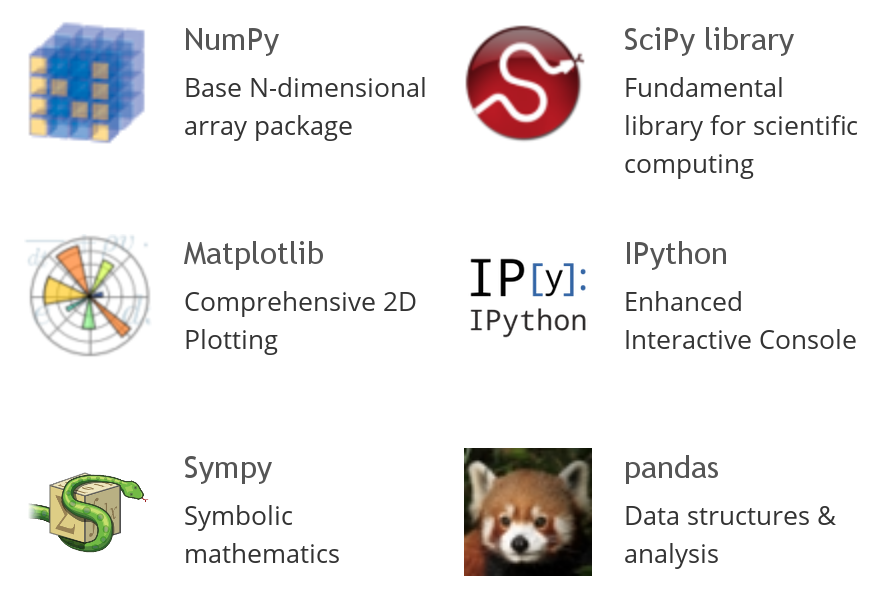
\includegraphics[width=0.7\textwidth]{SciPyEco}}%
  \only<2>{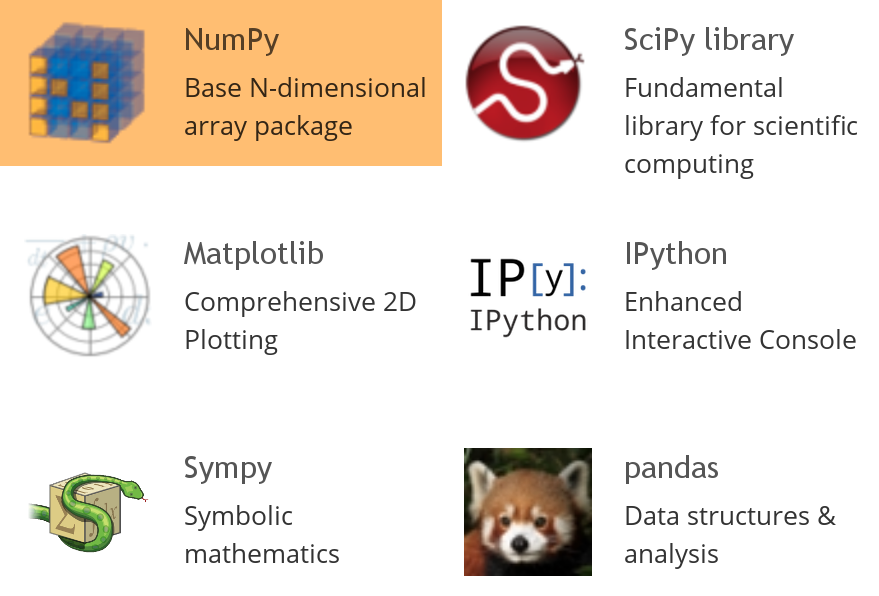
\includegraphics[width=0.7\textwidth]{SciPyEco_NumPy}}\quad%
  \raisebox{0.2truecm}{%
   \begin{sideways}
    \tiny from: \url{www.scipy.org}
   \end{sideways}}
 \end{center}

 + SciKits and many other packages
}

\frame
{
 \vspace*{-0.5truecm}
 \begin{columns}
  \begin{column}[t]{0.5\textwidth}
   \begin{center}
    \structure{www.scipy-lectures.org}

    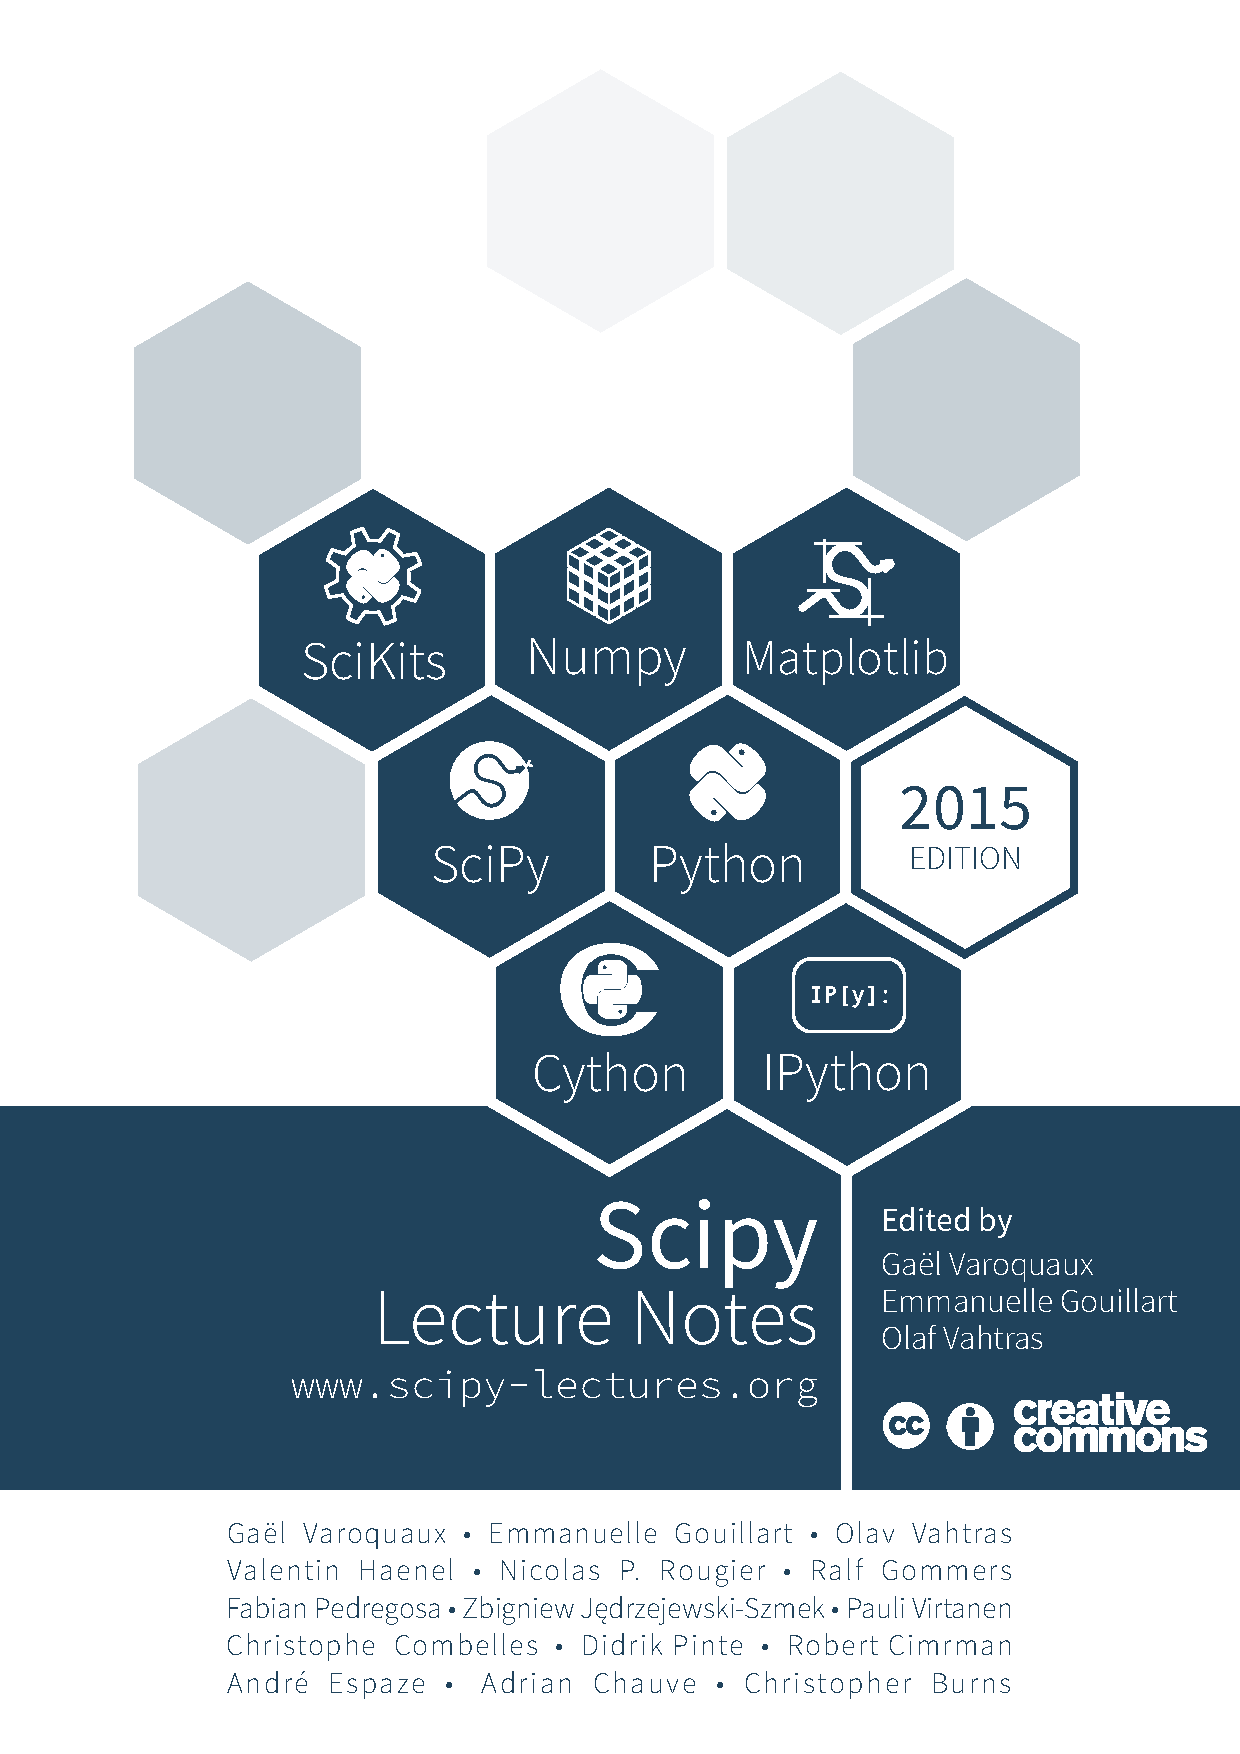
\includegraphics[width=\textwidth]{ScipyLectCover}
   \end{center}
  \end{column}%
  \begin{column}[t]{0.5\textwidth}
   \begin{center}
    \structure{docs.scipy.org/doc/numpy/}

    \vspace{0.3truecm}
    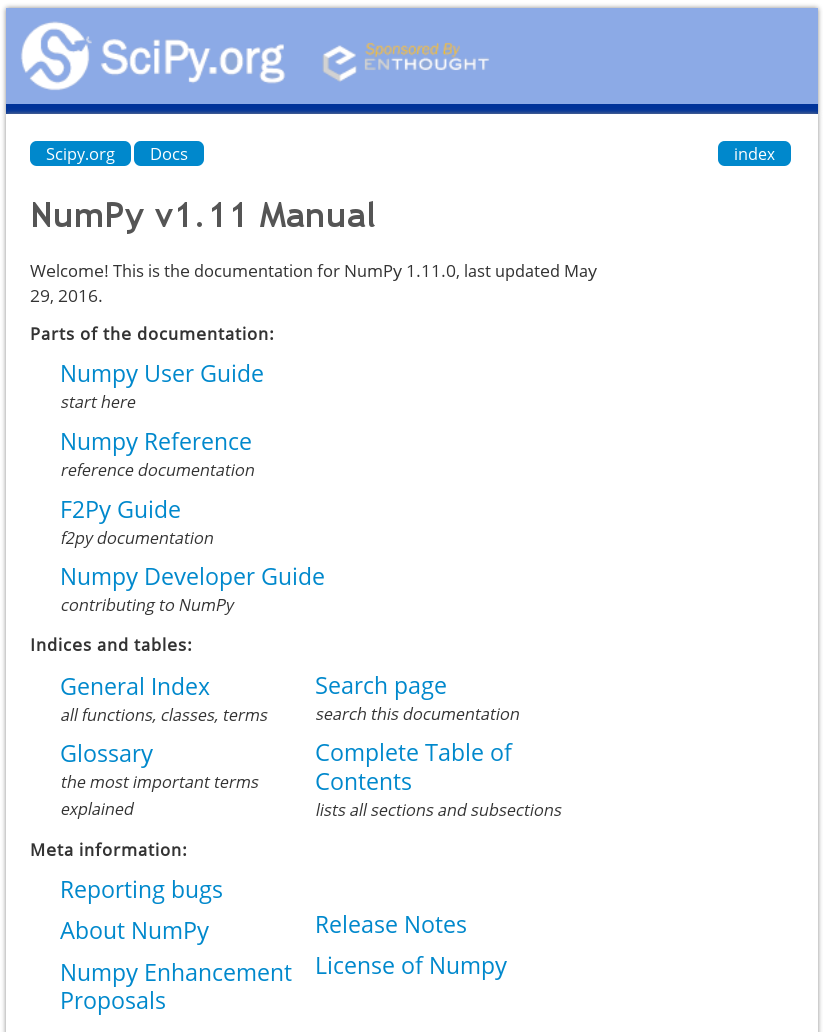
\includegraphics[width=\textwidth]{NumpyManual}
   \end{center}
  \end{column}
 \end{columns}
}

\frame
{
 \frametitle{A wish list}

 \begin{itemize}
  \item we want to work with vectors and matrices
 \end{itemize}

 \begin{columns}
  \begin{column}{0.55\textwidth}
   \begin{displaymath}
    \begin{pmatrix}
     a_{11} & a_{12} & \cdots & a_{1n}\\
     a_{21} & a_{22} & \cdots & a_{2n}\\
     \vdots & \vdots & \ddots & \vdots\\
     a_{n1} & a_{n2} & \cdots & a_{nn}\\
    \end{pmatrix}
   \end{displaymath}
  \end{column}%
  \begin{column}{0.45\textwidth}
   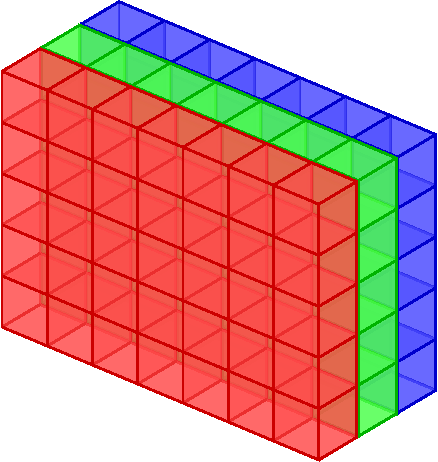
\includegraphics[width=0.7\textwidth]{rgbarray}

   colour image as $N\times M\times3$-array
  \end{column}
 \end{columns}

 \begin{itemize}
  \item we want our code to run fast
  \item we want support for linear algebra
  \item \dots 
 \end{itemize}
}

\frame
{
 \frametitle{List indexing and slicing}

 \begin{center}
  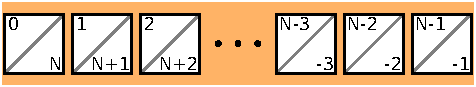
\includegraphics[width=0.96\textwidth]{listindexing2}

  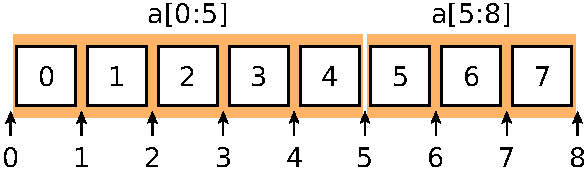
\includegraphics[width=\textwidth]{listindexing1}
 \end{center}
}

\end{document}
